
\chapter[System Design]{System Design}{System Design}\label{sd}

\noindent
\rule{0.49\textwidth}{0.75pt} $_{\bigcirc}$ \rule{0.49\textwidth}{0.75pt}\\

\section{Design Diagrams}

\subsection{Data Flow Diagram}
 \begin{figure}[h!]
     \centering
     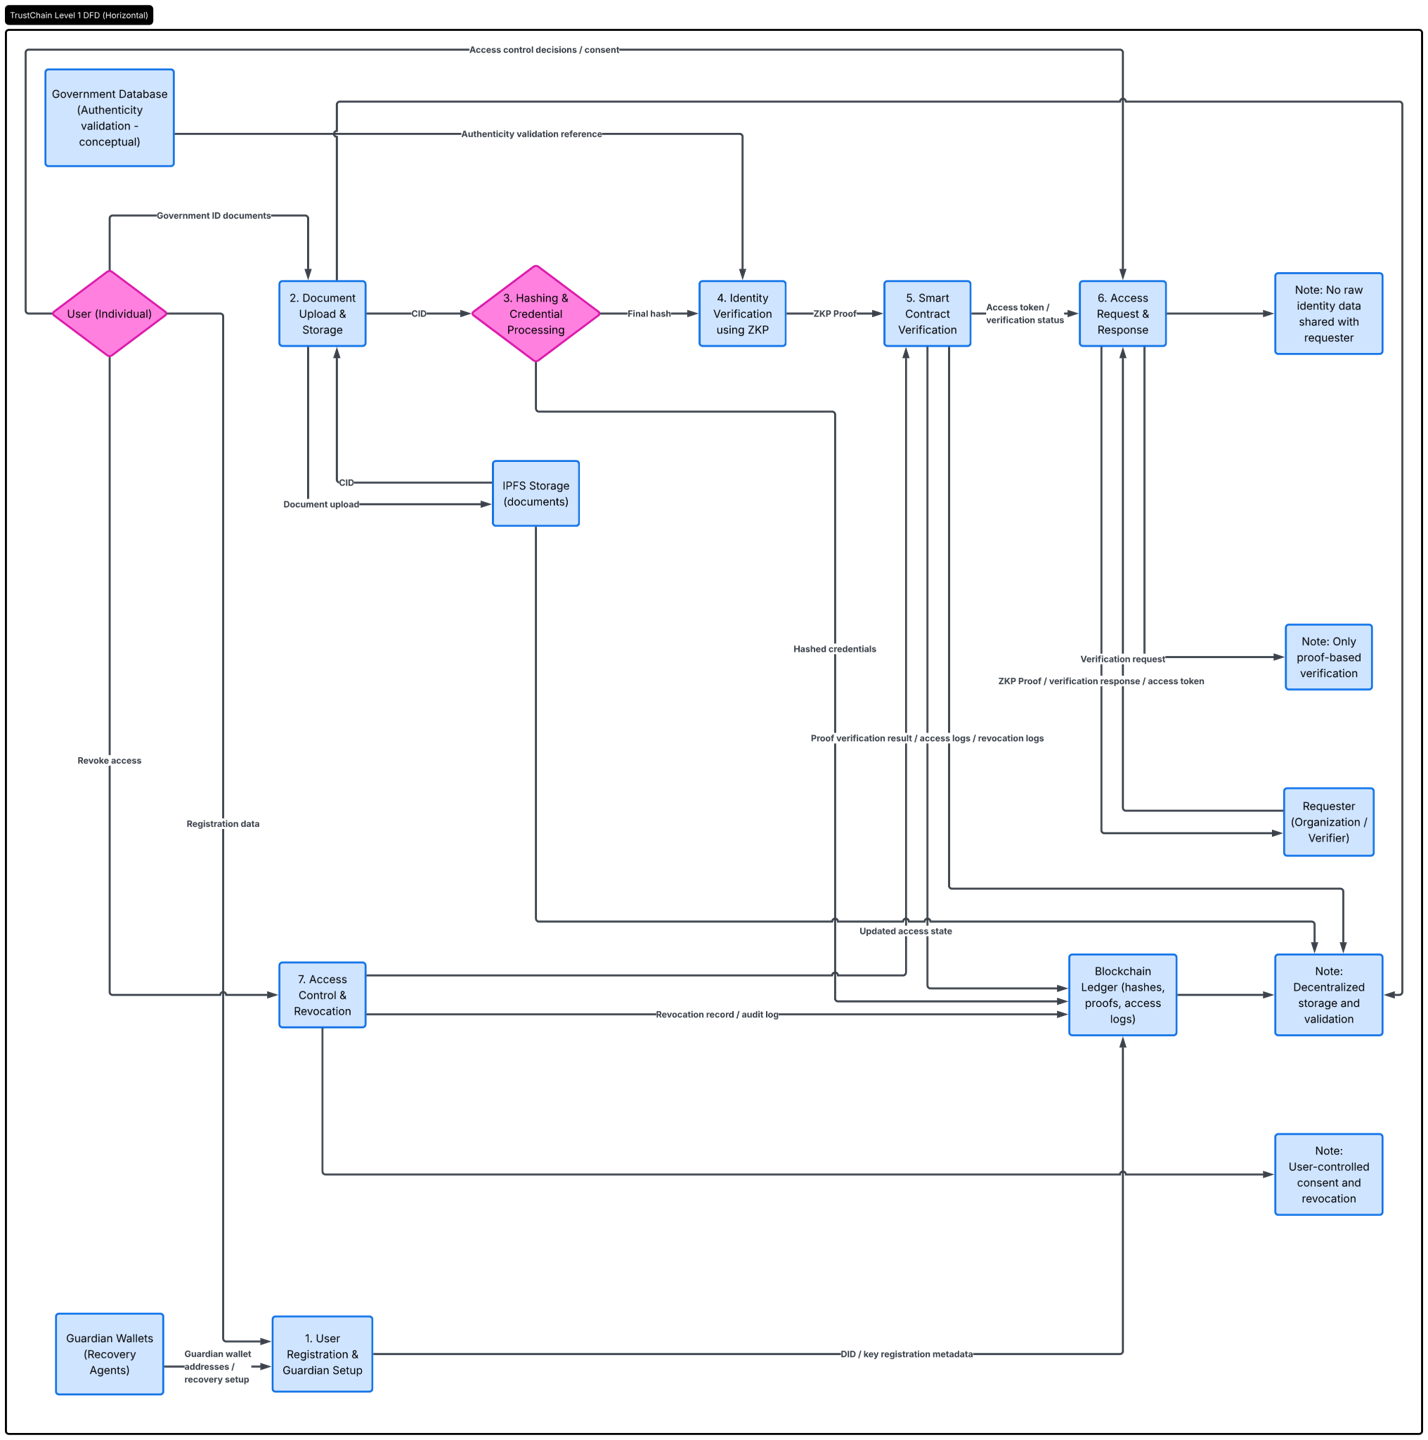
\includegraphics[width=1\textwidth]{Chapter1/DFD.png} % Adjust the width as needed
     \caption{Data Flow Diagram}
     \label{f1} 
\end{figure}
Data Flow Diagram of TrustChain is the general flow of data in the system showing the processing of the identity information safely without exposing it. In the diagram, interaction is shown between user entities and the internal processes of the system and the decentralized elements of IPFS and blockchain. It distinctly outlines the movement of data (between registration and verification) by maintaining privacy control and integrity at all levels of the system design and implementation. This framework can be used to comprehend secure communication and system dependencies.

The flow chart starts with the registration of users and guardians in which members input necessary information and allocate recovery wallets. Such wallets serve as trustworthy sources that allow the restoration of accounts and keep control in the event of loss of access. The information on registration is fed into the system that triggers the creation of identity and its connection to decentralized identifiers and cryptography keys that guarantee ownership and secure authentication throughout the platform. It also lays the foundation of initial trust relations needed in subsequent verification processes in system flow.

Users register with their identity documents that are kept on IPFS with decentralized storage system. The system creates a content identifier of every document and it is processed with multi layer hashing with keccak based operation. This provides assurance that no unprocessed document is ever exposed and integrity is maintained and allows the secure work process across constituents. The hashes generated are processed to derive proofs and check that they are consistent.

Then the diagram shows how identity verification can be done with Zero Knowledge Proofs where hashed credentials are verified without disclosing sensitive information. The mechanism of ZK STARK guarantees cryptographic security and avoids trusted setup. These evidences are then provided to smart contracts deployed on the blockchain that execute verification logic and impose role based access control. The blockchain stores hashes proofs and access logs that guarantee the transparency immutability and auditability of any operation, conducted in the system. This measure enhances inter-party trust and ensures high- privacy standards throughout interactions.

Lastly the access request and response process enables the requesters to authenticate identity with proof based validation as opposed to accessing real documents. Users are in full control of their data by giving or withdrawing permissions anytime during interactions with smart contracts. Every activity is documented on the blockchain which guarantees irreversible records and responsibility. The diagram focuses on decentralized storage user permission and secure validation that ensure the system is scalable and reliable to be implemented in the real world identity verification applications. It also emphasizes connectivity between frontend backend and blockchain layers that guarantee a smooth flow of data and efficiency of operation.





\subsection{Use Case Diagram}


\begin{figure}[h!]
    \centering
    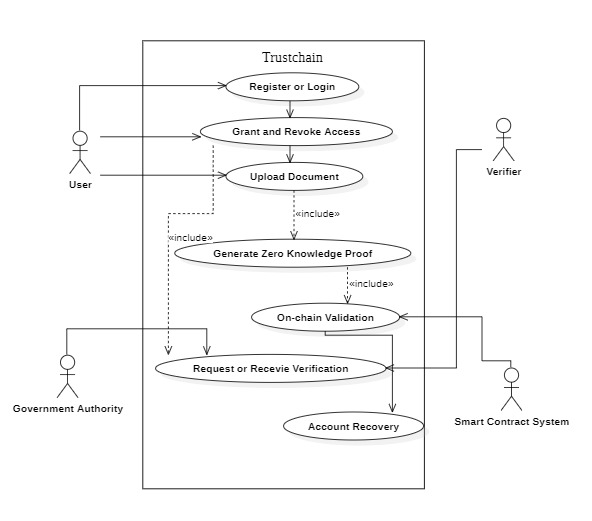
\includegraphics[width=1\textwidth]{Chapter1/use_case_new.jpeg} % Adjust the width as needed
    \caption{Use Case Diagram }
    \label{f1} % Optional: for referencing the figure in your document
\end{figure}
The Use Case Diagram of TrustChain shows how the various actors and the system interact with each other, in this case emphasizing the manner in which identity verification can be carried out without exposing sensitive data. It emphasizes the user centric control, secure identification and decentralized verification protocol. The diagram also clearly illustrates the boundaries of the systems, and the participation of each actor in the life cycle of identity within the platform.

The key players of the system are the User, Requester and Guardian Wallets. The User communicates with the system to register, upload and get access to documents. The Requester sends verification requests to verify identity without access to raw documents. Guardian Wallets are recovery agents, which guarantee safe account recovery. All the actors have well defined roles that aid in ensuring system security, reliability and user control during identity verification process.

The user can get started by registering on the site and creating guardian wallets to recover them. Once onboarded successfully the user uploads identity documents once. Such documents are safely stored and manipulated in the system to create verifiable credentials and hashed representations to be verified further.

The requester engages the system by making a verification request. The system does not handle real identity documents but instead does the request based on cryptographic proofs. The user is alerted and he can approve or reject. This guarantees verification is carried out at the consent of the user and the full privacy of sensitive information.

It has several processes that are done internally such as hashing and Zero Knowledge Proof generation and validation of smart contracts. All these mechanisms combine and authenticate identity without exposing personal information. An access control is implemented with the help of smart contracts on the blockchain where permissions can be granted and denied. All the interactions are documented to maintain transparency and traceability as well as to secure and efficient verification workflows.

Altogether, the Use Case Diagram focuses on a privacy first design, in which the users will be in charge of their identity information. It shows how TrustChain is used to substitute the traditional document sharing with the use of proof based validation. Secure interactions among actors as well as system components to guarantee a scalable, reliable and user friendly identity verification solution are also emphasized in the diagram.


\subsection{Data Structure Design and Smart Contract}
The TrustChain Smart Contract and Data Structure Design eliminates the necessity of a conventional database schema and uses the blockchain and decentralized storage systems. Rather than having centralized systems holding raw identity data, the architecture concentrates on having structured references like hashes, proofs and access states. This will make sure that no sensitive information is directly exposed, at the same time making it possible to effectively verify identity. The architecture is a hybrid in that, critical verification information is stored on chain, and real documents are off chain in IPFS.

Smart contracts serve as the first layer in the system of data management. They take care of storing hashed credentials, decentralized identifiers and upholding access control logic. Every user is linked to a distinctive identity framework comprising of hashed document references and permission states. Verification requests, responses and revocation actions are also documented in the contracts. This organised method also guarantees immutability, traceability and safe management of identity related processes without the use of central databases.

Integration of IPFS compliments blockchain as it deals with storage of documents in a decentralized fashion. The smart contracts only contain links to content identifiers and hashes derived, providing integrity without revealing raw content. Access logs and proof validation records that make data structure also allow auditability. This architecture guarantees scalability, privacy and effective data processing.


\rule{0.49\textwidth}{0.75pt} $_{\bigcirc}$ \rule{0.49\textwidth}{0.75pt}\\
